\documentclass[english]{article}
\usepackage[T1]{fontenc}
\usepackage[utf8]{luainputenc}
\setcounter{secnumdepth}{4}
\setcounter{tocdepth}{4}
\usepackage{color}
\usepackage{babel}
\usepackage{array}
\usepackage{graphicx}
\usepackage{setspace}
\usepackage{todonotes}
\usepackage{placeins}
\usepackage[tocentry, tablegrid,nochapter]{vhistory} 
\usepackage{catchfilebetweentags}
\usepackage{adjustbox}
\usepackage{float}
\usepackage{mathtools}
\usepackage{soul}
\usepackage{enumitem}
\usepackage{subfigure}


\usepackage{pgfgantt,rotating}
\definecolor{barblue}{RGB}{153,204,254}




\usepackage[unicode=true,
bookmarks=true,bookmarksnumbered=true,bookmarksopen=false,
breaklinks=false,pdfborder={0 1 1},backref=false,colorlinks=false]
{hyperref}
\hypersetup{pdftitle={ITPD},
	pdfauthor={Piazzolla Matteo Michele - Millimaggi Andrea},
	pdfsubject={Testing}}

\usepackage{fancyhdr,graphicx,lastpage}% http://ctan.org/pkg/{fancyhdr,graphicx,lastpage}
\fancypagestyle{plain}{
	\fancyhf{}% Clear header/footer
	\fancyhead[L]{Project Plan }% Right header
	\fancyhead[R]{\emph{Issue 1}}% Right header
	\fancyfoot[L]{Piazzolla Matteo Michele - Millimaggi Andrea}% Left footer
	\fancyfoot[R]{\thepage\  / \pageref{LastPage}}% Right footer
}
\pagestyle{plain}% Set page style to plain.


\makeatletter

\providecommand{\tabularnewline}{\\}

%%%%%%%%%%%%%%%%%%%%%%%%%%%%%% Textclass specific LaTeX commands.
\newcommand{\lyxrightaddress}[1]{
	\par {\raggedleft \begin{tabular}{l}\ignorespaces
			#1
		\end{tabular}
		\vspace{1.4em}
		\par}
}

\usepackage[font=small,labelfont=bf]{caption}

%%%%%%%%%%%%%%%%%%%%%%%%%%%% alloy listing



\usepackage{listings}


%%%%%%%%%%%%%%%%%%%%%%%%%%%% tabella dei vari issue 
\newcommand{\revisionhistory}{
	
	\begingroup
	\fontsize{15pt}{12pt}\selectfont
	\textbf{Revision History}
	\endgroup
	
	\begin{versionhistory}
		\vhEntry{1.0}{13/11/16}{Piazzolla  Millimaggi }{First document issue}
		\vhEntry{ }{ }{ }{ }
		\vhEntry{ }{ }{ }{ }
\end{versionhistory}}
\usepackage{xstring}
\newcommand{\fprow}[3]{
	\textbf{#1} &  \IfEqCase{#2}{%
		{0}{Simple}%
		{1}{Medium}%
		{2}{Complex}%
	} & #3 \tabularnewline \hline
}

\newcommand{\fptable}[2]{
	\begin{center}
		\begin{adjustbox}{max width=\textwidth}	
			\begin{tabular}{|c|c|c|}
				\hline 
				\textbf{Data} &  \textbf{Weight Type }& \textbf{Weight} \tabularnewline
				\hline 
				\hline 
		#1
				\textbf{TOT} & \multicolumn{2}{c|}{\textbf{#2}}\tabularnewline \hline
			\end{tabular}
		\end{adjustbox}	
		\par\end{center}
}


\def\arraystretch{1.5}%  1 is the default, change whatever you need


\makeatother

%%%%%%%%%%%%%%%%%%%%%%%%%%%% inizio documento
\begin{document}
	
	\title{
\includegraphics[scale=0.4]{img/polimi}\\
		Computer Science and Engineering}
	
	\begin{doublespace}
		
		\author{A.A. 2016/2017\\
			Software Engineering 2 Project: \\
			\\
			{\LARGE{}``PowerEnJoy''}\textbf{}\\
			\\
			\textbf{P}roject \textbf{P}lan \\
		}
	\end{doublespace}
	
	\maketitle
	\thispagestyle{empty}
	\lyxrightaddress{Prof.Luca Mottola\\
		\\
		Matteo Michele Piazzolla Matr. 878554\\
		Andrea Millimaggi Matr. 876062}
	
	%%%%%%%%%%%%%%%%%%%%%%%%%%%%
	\newpage
	
	
	
	%%%%%%%%%%%%%%%%%%%%%%%%%%%%
	
	
	\revisionhistory
	
	%%%%%%%%%%%%%%%%%%%%%%%%%%%%
	\newpage{}
	
	\tableofcontents{}
	
	%%%%%%%%%%%%%%%%%%%%%%%%%%%%
	\newpage
	
	\listoftodos
	%%%%%%%%%%%%%%%%%%%%%%%%%%%%
	\newpage
	
	\listoffigures
	
	%%%%%%%%%%%%%%%%%%%%%%%%%%%%
	\newpage{}


	\section{INTRODUCTION}
\subsection{Purpose and Scope}
\subsubsection{Purpose}
The purpose of this document is to provide an estimation of the cost and the size of the project. This knowledge is needed to organize the resources needed in the development of the system and to properly schedule the activities of the project.\newline
To reach this purpose, two models will be used:
\begin{itemize}
\item \textbf{Function Point:} This approach is used to estimate the size of the project in LOC.
\item \textbf{COCOMO:} This model is used to estimate the effort required by the project in PM.
\end{itemize}

\subsubsection{Scope}
PowerEnJoy is a digital system for the management of a car-sharing service that only employs electric cars. In particular the aim is to develop a mobile application that allows the user to pick up and use electric cars in the areas reached by the service.

\subsection{List of Definitions and Abbreviations} 
\subsubsection{Acronyms}
\begin{itemize}
\item RASD: Requirement Analysis and Specification Document.
\item DD: Design Document.
\item DBMS: Database Management System.
\item DB: Database.

\item GPS: Global Positioning System

\end{itemize}
\subsubsection{Definitions}

\subsubsection{Abbreviations}
\begin{itemize}
	\item  FP: Function Points.
	\item  ILF: Internal logic file
	\item  ELF: External logic file.
	\item  EI: External Input.
	\item  EO: External Output.
	\item  EQ: External Inquiries.
	\item PH: Person Hours.
	\item LOC: Lines Of Code.
\end{itemize}



\subsection{List of Reference Documents}
\begin{itemize}
	\item PowerEnJoy RASD.	
	\item PowerEnJoy DD.
	\textbf{NOTE:} The reader must refer to the version 1.1 of the DD.
	\item COCOMO II Model Definition Manual 
\end{itemize}


	\pagebreak
	\section{Function Points: size estimation}
\subsection{Overview}
We use the Function Points approach to estimate the size of the project. This approach makes an estimation of the size of the project based on the functionalities of the system. In particular it analyses:
\begin{itemize}
\item Data structures. These can be of two types:
	\begin{itemize}[label={-}]
	\item Internal Logic Files, that are logically related data which are used and managed by the application.
	\item External Interface Files, that are logically related data which are used by the application, but are generated, reside and are managed in other applications.
	\end{itemize}
\item External Input operations, that are operations that elaborate data coming from external systems
\item External Output operations, that are operations that generate data to send to external systems .
\item External Inquiries, that are operations that involve both input and output and allow to retrieve data from Internal Logic Files and External.
\end{itemize} 
To each element of those types a weight is given, based on the complexity of the table.\newline
Multiplying the elements by their weights and summing the results we obtain the overall Function Points:\newline

\begin{equation}
FP = \sum_{}{}{Number\hspace{0.1 cm} of\hspace{0.1 cm} elements\hspace{0.1 cm} of\hspace{0.1 cm} a\hspace{0.1 cm} type * weight} 
\end{equation}

At the end, using the number of FPs, an estimation of the LOC of the project is estimated with the following formula:
\begin{equation}
LOC = AVC * number\hspace{0.1 cm} of\hspace{0.1 cm} function\hspace{0.1 cm} points
\end{equation}

AVC is a parameter that depends on the programming language used. We have chosen to use the Average value for Java among the values of the table that can be found in \cite{AVCTable}, because Java is the main language used in the project. 

\begin{figure}[h]
	\centering
	\subfigure[FP Counting Weights]{\label{fig:fp_counting}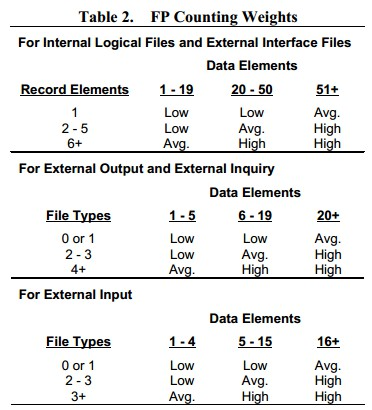
\includegraphics[width=60mm]{img/fpcounting.jpg}}
	\subfigure[UFP Complexity Weights]{\label{fig:fp_total}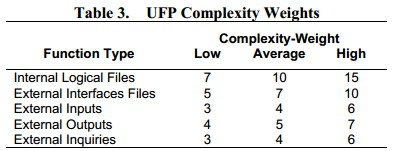
\includegraphics[width=60mm]{img/fptotal.jpg}}
	\caption{FP Analysis}
\end{figure}
\FloatBarrier


\subsection{Internal Logic Files} 

The PowerEnjoy Service needs to store information about:

\begin{itemize}
	\item \textbf{User:} This data consist in a small set of user information, for this reason its complexity has been considered \textbf{Simple}
	\item \textbf{Car:} This data consist in a small set of car information, for this reason its complexity has been considered \textbf{Simple}
	\item \textbf{Safe Area:} This data consist in a small set of safe area information, for this reason its complexity has been considered \textbf{Simple}
	\item \textbf{Trip:} This data consist in a small set of trip information, for this reason its complexity has been considered \textbf{Simple}
\end{itemize}
\fptable{			
	\fprow{User}{0}{7}	
	\fprow{Car}{0}{7}	
	\fprow{Safe Area}{0}{7}
	\fprow{Trip}{0}{7}
}

\subsection{External Interfaces File} 

\begin{itemize}
	\item \textbf{GPS positioning:} This data consist on information received by user or by OnBoard device of the car. \\Because the managing involve some algorithms it's considered \textbf{High}
\end{itemize}

\fptable{			
	\fprow{GPS positioning}{2}{10}	
}

\subsection{External Input} 
\begin{itemize}
	\item \textbf{Sign-Up:} Create a new user entry in the system Database. \\The complexity has been considered \textbf{Simple}
	\item \textbf{Log-In/Log-Out:} Manage the user authentication. Require a module to generate an auth token\\The complexity has been considered \textbf{Medium}
	\item \textbf{Update user information:} Update users information in the system Database. \\The complexity has been considered \textbf{Simple}
	\item \textbf{Request car reservation:} Manage the car reservation in the system. Require many check on the availability.  \\The complexity has been considered \textbf{Medium}
	\item \textbf{Unlock car:} Check if the user is nearby the reserved car and send an unlock request to the car. Require algorithm on user position.  \\The complexity has been considered \textbf{Complex}
\end{itemize}

\fptable{			
\fprow{Sign-Up}{0}{3}	
\fprow{Log-In/Log-Out}{1}{4}	
\fprow{Update user information}{0}{3}	
\fprow{Request car reservation}{1}{4}	
\fprow{Unlock car}{2}{6}
}

\subsection{External Inquiries} 
A PowerEnJoy user can ask the system for the retrieval of some data:
\begin{itemize}
\item \textbf{Car list:} User can request the list of cars available in a certain area or address. Involve Geolocalization algorithms.  \\The complexity has been considered \textbf{Medium}
\item  \textbf{Special Parking Area request:} User can request the list of available special parking areas. Require to query the status of the nearby special parking area.\\The complexity has been considered \textbf{Medium}
\item  \textbf{Parking Area request:} User can request the list of parking areas. Require to query the status of the nearby special parking area. \\The complexity has been considered \textbf{Medium}
\item  \textbf{Personal Data request:} User can request to see its personal data. Data can be obtained with a simple Database Query. \\The complexity has been considered \textbf{Simple}
\item  \textbf{Trip list:} User can request the list of trips done in a certain period.\\
The complexity has been considered \textbf{Complex}
\end{itemize}

\fptable{			
	\fprow{Car list}{1}{4}
	\fprow{Special Parking Area request}{1}{4}
	\fprow{Parking Area request}{1}{4}
	\fprow{Personal Data request}{0}{3}
	\fprow{Trip list}{2}{6}
}

\subsection{External Output} 
Beyond answers to External Inquiries, the system has to send other types of messages to the user:
\begin{itemize}
\item \textbf{Reservation confirmation:} A notification of the confirmation of a reservation. Require email or push notification system. \\The complexity has been considered \textbf{Simple}
\item \textbf{End Trip notification:} A notification of the end of a trip. Require the status of the car through the OnBoard device \\The complexity has been considered \textbf{Medium}
\item \textbf{Payment notification:} A notification of the confirmation of the payment. Require an integration with the payment system \\The complexity has been considered \textbf{Medium}
\end{itemize}

\fptable{			
	\fprow{Reservation confirmation}{0}{4}
	\fprow{End Trip notification}{1}{5}
	\fprow{Payment notification}{1}{5}
}

\subsection{Results} 
According to the element in each section and their weight in complexity the total of  Function Points that provide an indication of the size of the system in functional terms:

\begin{equation}
FP=ILF+EIF+EI+EQ+EO 
\end{equation}

Total Function Points: \textbf{\arabic{total_fp}}


Using 46 as AVC the final value of the estimated line of code is:

\begin{equation}
LOC = 46 * 93 = 4278
\end{equation}

	\pagebreak
	\section{COCOMO analysis}
The COCOMO model allows to estimate the time effort required by the project. We use the version of this model called COCOMO II. It is based on a main formula:
\begin{equation}
PM = A * Size^{E} * \prod_{1<=i<=n}^{} EM_{i} 
\end{equation}

where:
\begin{itemize}
	\item \textbf{PM} stands for "Person-Months"
	\item \textbf{A}=2.94. It approximates a productivity constant in PM/KSLOC for the case where E = 1.0.
	\item \textbf{Size} is measured in KSLOC and is the result of the Function Points analysis.
	\item \textbf{E} is an aggregation of 5 \textbf{scale factors}:
	\begin{itemize}[label = {-}]
		\item \textbf{Precedentedness:} It is high if the project is similar to several previous projects
		\item \textbf{Development Flexibility:} It is high if there are no specific constraints to conform to pre-established     requirements and external interface specifications.
		\item \textbf{Architecture/Risk Resolution:} It is high if the project plan includes a good risk management plan, a clear definition of budget and schedule, with a focus on architectural definition
		\item \textbf{Team Cohesion:} It is high if all stakeholders are able to work in a team and share the same vision and commitment.
		\item \textbf{Process Maturity:} Refers to a well known method for assessing the maturity of a software organization, CMMI, that is a process level improvement training and appraisal program.
	\end{itemize}
	\begin{figure}[H] 
		\centering
		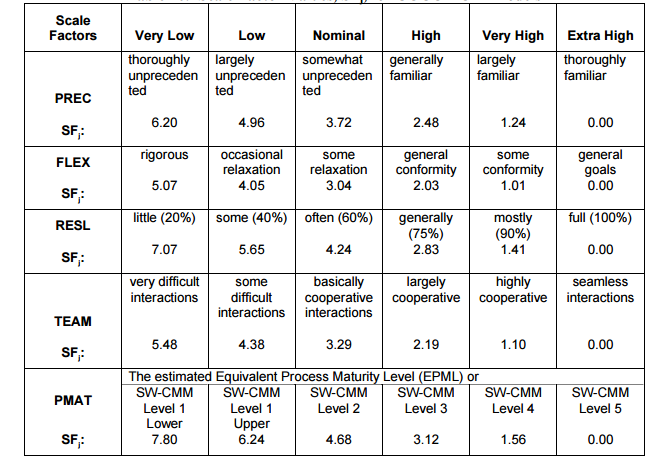
\includegraphics[scale = 0.7]{img/scaleFactors.png}
		\caption{Scale Factors}
	\end{figure}
	
	E is calculated with the formula:
	\begin{equation}
	E = B + 0.01 * \sum_{1<=j<=5}^{} SF_{j}
	\end{equation}
	where B=0.91
\end{itemize}


\subsection{Scale Factors}
\subsubsection{Precedentedness}
For our development team is the first project done in the field of Car Sharing involving electric cars and so the personnel has no previous knowledge about it. For this reason we consider the Precedentedness of our project \textbf{Very low}.\\
\textbf{PREC=6.20}

\subsubsection{Development Flexibility}
As for pre-established requirements, the development team is provided with a lot of requirements about the application and the service to be considered. On the other hand, there is no constraint on external interfaces to be considered.
So, taking the average of the low flexibility for requirements and the high flexibility on external interfaces, the resulting Development Flexibility is \textbf{Nominal}.\\
\textbf{FLEX=3.04}

\subsubsection{Architecture/Risk Resolution}
Considering that the people in charge of project planning are new to this job, but they are also very motivated and able to learn fast, we can consider that their work on the risk management plan and the definition of budget and schedule has a \textbf{Nominal} rate, taking the average of the low experience and the personnel characteristics.\\
\textbf{RESL=4.24}

\subsubsection{Team Cohesion}
The group working on the project has newly been assembled, so its cohesion is in general unknown. Nevertheless, the people selected to join the group are all young, motivated, open-minded and suitable for group-works, so we can consider the Team Cohesion \textbf{Nominal}, taking the average of high uncertainty and good skills of the personnel.\\
\textbf{TEAM=3.29}

\subsubsection{Process Maturity}
The maturity level of the project is \textbf{2}, for this reasons:

\begin{itemize}
	\item The processes of our project will be planned and executed according to specific and clear criteria. 
	\item The people that will work on the project have been selected among a wide list of candidates and only the one that have demonstrated to have the best skills have been chosen.
	\item We consider the resources provided by the customer and the ones already owned by the development team adequate.
	\item We have the purpose of involving in the processes all the stakeholders as much as possible, to have frequent feedbacks and suggestions on the works
	\item Having the purpose of receiving feedbacks, we will use them and other evaluations to check the adherence of the project to requirements.
	\item The development team is focused only on the PowerEnJoy project, so of course the processes are planned, documented, performed,monitored and controlled at the project level.
	\item Because the development team has no previous knowledge about the field of car sharing, it will have mainly a reactive behavior, because it cannot predict problems that it doesn't know.  
\end{itemize}  
\textbf{PAMT=4.68}

\pagebreak
\subsection{Effort Multiplier}
\textbf{EM} stands for Effort Multiplier. Effort multipliers are derived from \textbf{Cost drivers}. The selection of these cost drivers depends on wh1ether the project regards a \textbf{Post-Architecture} system or a \textbf{Early Design} system. We are in the Early Design case, because we are extending an existing product and our system will be developed from scratch. So the cost drivers are:

\subsubsection{Personnel Capability}
Personnel Capability (PERS) is a combination of Analyst Capability(ACAP), Programmer Capability(PCAP) and Personnel Continuity cost driver of Post-Architecture.\\
In our case we have little experience in the software analysis but this is balanced by good programming skills. The combination of ACAP and PCAP can be considered as \textbf{"Nominal"}
\textbf{PERS=1.0}
\begin{figure}[H] 
	\centering
	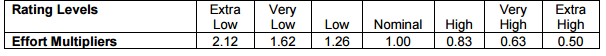
\includegraphics[scale = 0.6]{img/PERS.png}
	\caption{EMs of PERS}
\end{figure}
		

			
\subsubsection{Product Reliability and Complexity}
	Product Reliability and Complexity(RCPX) is a combination of Required Software Reliability(RELY), Data Base Size(DATA), Product Complexity(CPLX) and Documentation Match to Life-Cycle Need(DOCU) cost drivers of Post-Architecture. 
			\\
			The software reliability is very important because a failure of the system can potentially cause a huge financial loss.\\
			The DATA cost driver attempts to capture the effect large test data requirements have on product development. For this particular driver we don’t have enough information to do a reliable estimation so the value can be considered \textbf{"Nominal"}.\\
			We decided to assign the complexity of the system a value \textbf{"High"}
\\
\textbf{RCPX=1.33}

\begin{figure}[H] 
	\centering
	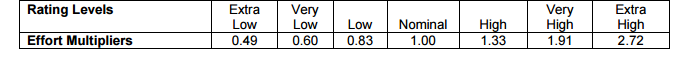
\includegraphics[scale = 0.6]{img/RCPX.png}
	\caption{EM of RCPX}
\end{figure}
	
		
\subsubsection{Developed for Reusability}		
		There are no requirement on Reusability so the value is considered \textbf{"Nominal"}
\\
\textbf{RUSE=1.0}
			
		\begin{figure}[H] 
			\centering
			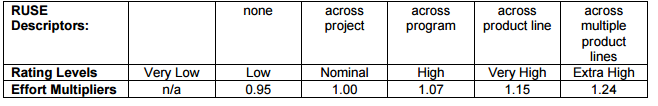
\includegraphics[scale = 0.6]{img/RUSE.png}
			\caption{EMs of RUSE}
		\end{figure}

\subsubsection{Platform Difficulty}		
Platform Difficulty (PDIF) is a combination of Execution Time Constraint(TIME), Main Storage Constraint(STOR) and Platform Volatility(PVOL) cost drivers of Post-Architecture. 
		\\
		The OnBoard device is real-time embedded product so the execution time is important, but on the rest of the system there are no particular constraint about the execution time. Same as before there are no requirements on Storage so both can be considered ad \textbf{"Nominal"}.
		Platform Volatility can be considered \textbf{"Very high"} because the system is composed of different part on different system (OnBoard Device, Application Logic on server, Client on smartphone or browser).
		\\
		\textbf{PDIF=1.29}
		
		\begin{figure}[H] 
			\centering
			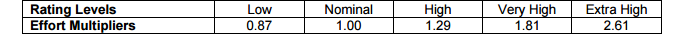
\includegraphics[scale = 0.6]{img/PDIF.png}
			\caption{EMs of PDIF}
		\end{figure}
	
\subsubsection{Personnel Experience}		
{Personnel Experience (PREX) is a combination of Application Experience(APEX), Platform Experience(PLEX), Language and Tool Experience(LTEX) cost drivers of Post-Architecture. 
			\\
			Because of the team inexperience the overall value is considered \textbf{"Low" }
			\\
			\textbf{PREX=1.22}
		\begin{figure}[H] 
			\centering
			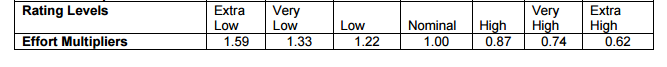
\includegraphics[scale = 0.6]{img/PREX.png}
			\caption{EMs of PREX}
		\end{figure}

\subsubsection{Facilities }		
Facilities (FCIL) is a combination of Use of Software Tools(TOOL) and Multisite Development(SITE) cost drivers of Post-Architecture. 
		\\
		Because of the entity and the life-cycle of the product development there are different system and tools that need to be integrated to develop the whole product so TOOL is considered \textbf{"Low"}.
		With all the new collaboration tools (Slack, github, Skype) the Multi-Site development driver is considered \textbf{"Nominal"}
		\\
		\textbf{FCIL=1.10}
		\begin{figure}[H] 
			\centering
			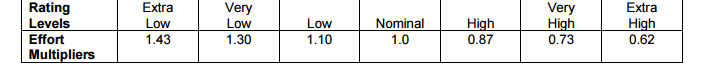
\includegraphics[scale = 0.6]{img/FCIL.png}
			\caption{EMs of FCIL}
		\end{figure}

\subsubsection{Required Development Schedule }		
	Required Development Schedule (SCED):
		\\
		Non accelerated Waterfall Developement Schedule so it's considered \textbf{"Nominal"}.
		\\
		\textbf{SCED=1.0}
		
		\begin{figure}[H] 
			\centering
			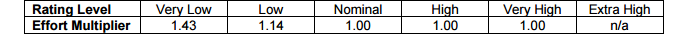
\includegraphics[scale = 0.6]{img/SCED.png}
			\caption{EMs of SCED}
		\end{figure}
	



\begin{table}[H]
	\centering
	\resizebox{\textwidth}{!}{%
		\begin{tabular}{lllllllll}
			\hline
			\textbf{Driver} & PERS & RCPX & RUSE & PDIF & PREX & FCIL & SCED & Product   \\ \hline
			\textbf{Value}  & 1.0  & 1.33 & 1.0  & 1.29 & 1.22 & 1.10 & 1.0  & 2.3024694 \\ \hline
		\end{tabular}%
	}
	\caption{EM Result Table}
\end{table}

\FloatBarrier

\subsection{Results} 
According to the Scale Factors and the Effort Multiplier

$$Effort = A * KLOC^{E} * EAF$$
$$A=2.94$$
$$EAF=\prod_{1<=i<=n}^{} EM_{i} \approx2.3$$
$$E=0.91+0.01*21.45$$
\\
Total effort result in persons months:
$$PM = 34.70$$

%1,33*1,29*1,22*1,1=2,3024694

\begin{equation}
Duration = 3.67 * (PM)^{(0.28+0.2 * (E - 0.91))} = 11.4924
\end{equation}
This equation brings us to a estimated duration of approximately 11.5 months.
\begin{equation}
Number of developers = \frac{Effort}{Duration} \approx3
\end{equation}
This brings to an estimation of 3 developers to allocate to this project.



	\pagebreak
	\section{Resources Allocation}
Through a Gantt chart, all activities are represented for blocks over time in order to highlight how resources are allocate to the various tasks. The beginning and the end of the block correspond to the beginning and at the end of the activity. Start of some activities are linked to the end of other.
\\
	\begin{center}
\begin{sideways}

\begin{ganttchart}[
	y unit title=0.5cm,
	y unit chart=0.5cm,
	vgrid={ dotted},
	time slot format=isodate,
	compress calendar,
	today={\the\year-\the\month-\the\day}, 
	title/.append style={shape=rectangle, fill=black!10},
	title height=1,
	bar/.append style={fill=green!90, rounded corners=3pt},
	bar height=.45,
	bar label font=\normalsize\color{black!50},
	group top shift=.6,
	group height=.3,
	group peaks height=.2,
	bar incomplete/.append style={fill=green!40},	
	]{2016-08-01}{2018-05-31}
	\gantttitlecalendar{year} \\
  \gantttitlecalendar{ month} \\



	\ganttset{progress label text={},
		bar incomplete/.append style={fill=green!40},
		group/.append style={draw=black, fill=green},} % this suppresses percentage done labels
	\ganttgroup{Requierements and Design}{2016-10-16}{2017-01-01} \\
	\ganttbar[progress=00, name=rasd]{Requirements Analysis}{2016-10-16}{2016-11-13} \\
	\ganttlinkedbar[progress=00, name=pdd]{Preliminary Design}{2016-11-13}{2016-12-11} \\
	\ganttbar[progress=00, name=itpd]{Integrated Test Plan}{2016-12-11}{2017-01-15} \\
	\ganttbar[progress=00, name=pp]{Project Plan}{2016-12-11}{2017-01-22} \\
	\ganttset{bar incomplete/.append style={fill=red!40},
		group/.append style={draw=black, fill=red}}
	\ganttgroup{Implementation}{2017-2-01}{2017-09-30} \\
	\ganttbar[progress=00, name=impl_database]{Database}{2017-02-01}{2017-03-31} \\
	\ganttbar[progress=00, name=impl_server]{Server Infrastructure}{2017-03-31}{2017-04-30} \\
	\ganttbar[progress=00, name=impl_backend]{Backend Logic}{2017-04-01}{2017-06-31} \\
	\ganttbar[progress=00, name=impl_obsw]{OnBoard Device Software}{2017-05-01}{2017-07-15} \\
	\ganttbar[progress=00, name=impl_app]{Mobile Application}{2017-07-01}{2017-09-30} \\
	\ganttbar[progress=00, name=impl_webd]{Website}{2017-07-01}{2017-09-30} \\
	\ganttset{bar incomplete/.append style={fill=blue!40},
		group/.append style={draw=black, fill=blue},}
	\ganttgroup{Testing}{2017-10-1}{2018-3-31} \\
	\ganttbar[progress=00, name=test_unit]{Unit Test}{2017-10-1}{2017-11-30} \\
	\ganttbar[progress=00, name=test_integration]{Integration Test}{2017-11-30}{2018-1-31} \\
	\ganttlinkedbar[progress=00, name=test_profiling]{Performance Test and Profiling}{2018-02-01}{2018-03-01} \\
	% misc links
	\ganttset{progress label text={}}

	\ganttlink[link mid=0.4]{pdd}{itpd}
	\ganttlink[link mid=0.2]{pdd}{pp}
	\ganttlink[link mid=0.3]{impl_database}{impl_backend}

\end{ganttchart}

\end{sideways}
\end{center}
	\pagebreak
	\section{Risk management}
In this section we mention the risks that could affect our project. We provide a brief description of the risk, its probability to actualize, the impact of such actualization on the project and possible solutions to take into account in order to avoid or limit the damages.
The possible values for the probability are \textit{Low, Medium} or \textbf{High}, while the possible values for the impact are \textit{Marginal, Serious} or \textit{Catastrophic}.
\subsection{Project Risks}
Project Risks are those risks which threaten the project plan and whose actualization can result in a slipping of the schedule \newline
\begin{adjustbox}{max width=\textwidth}
\begin{tabular}{|l|p{5 cm}|l|l|p{5 cm}|}
\hline
Risk & Description & Probability & Impact & Possible Solutions
\\ \hline
Personnel Shortfall & Due to a wrong estimation of the size of the project, there could be not enough people to complete the project deliveries in time & Medium & Serious & Prepare the personnel to the possibility of extra-work due to the lack of people. \newline Plan a possible new recruitment.	 
\\ \hline
Skill Lack & It could be the case that the team hasn't the skill required to face some types of issues, because it was not supposed to deal with them. & Low & Serious & Recruit people with more skills than the strictly required ones. \newline Consider the organization of update courses. 
\\ \hline
Size of the Project & The project size could be underestimated, because of the lack of knowledge about the field of the project  & Medium & Marginal & Prepare more resources than the strictly needed ones. \newline Consider a possible extension of the time of the project
\\ \hline
Competitors & Other companies can begin similar projects & Low & Serious & Plan an additional period in the schedule devoted to the development of new features and the improvement of the quality, in order to discourage the development of other similar projects
\\ \hline
Personnel Illness & People of the staff can be ill in critical phases of the project & High & Marginal & Make some tasks of the staff overlap with each other. In this way there will be always a possible substitute to ill people.
\\ \hline
 Data Loss & Data loss during the development & Low & Critical & Backup strategy and software versioning.
\\ \hline
\end{tabular}
\end{adjustbox}
\subsection{Technical Risks}
Technical Risks are those risks which threaten the quality and the functioning of the product and whose actualization makes the implementation more difficult. \newline
\begin{adjustbox}{max width=\textwidth}
\begin{tabular}{|l|p{5 cm}|l|l|p{5cm}|}
\hline
Risk & Description & Probability & Impact & Possible Solution
\\ \hline
Obsolete Design & Some new technology, that provides so as many better features to force the team to change the design of the system, could born in the course of the project & Low & Serious & Design the system in a way that allows to change components easily.
\\ \hline
Inadequate Infrastructure & The resources, the facilities and the machines provided by the company or owned by the team are discovered to be inadequate for the project & Low & Catastrophic & While defining the budget with the customer, ask him the creation of a fund for possible substitutions of inadequate equipment.
\\ \hline
New Requirements & New requirements are defined after the design phase& Low & Serious &The Waterfall development approach require frozen requirements. Change the to Scrum or Agile approach.

\\ \hline
\end{tabular}
\end{adjustbox}
\subsection{Business Risks}
Business Risks are those risks which threaten the feasibility of a complete product and the chances of selling it. Their actualization can cause bad results on sales and evaluation of consumers. \newline
\begin{adjustbox}{max width=\textwidth}
\begin{tabular}{|l|p{5 cm}|l|l|p{5 cm}|}
\hline
Risk & Description & Probability & Impact & Possible Solution
\\ \hline
Budget Lack & At some point it can be discovered that there has been an underestimation of the costs of project and that the budget is insufficient & Medium & Serious & Prepare a document to deliver to the customer, in which are explained the good results obtained till that moment, the reason for the budget increase, the disadvantages of non-concluding the project and the advantages of improving it with more functionalities.
\\ \hline
Market Risk & The team has developed a good product, but this does not match the real requirements, expectations and needs of consumers, resulting in poor sales & Medium & Catastrophic & Consider interviews to stakeholder and random consumers during all the phases of project in order to have feedbacks on the partial work done till a certain moment.
\\ \hline
\end{tabular}
\end{adjustbox}
	\pagebreak
	\section{Appendix}


	\subsection{Used software}
	\begin{enumerate}
		\item \textbf{TeXstudio:} \url{http://www.texstudio.org/} to redact this document in {\LaTeX} format.
		\item \textbf{Astah:} \url{http://astah.net/} to draw diagrams.		
	\end{enumerate}
	
	
	\subsection{Time effort}
	The estimated time spent by us to redact this document:
	\begin{center}
		\begin{adjustbox}{max width=\textwidth}	
			\begin{tabular}{|l|>{\raggedright}p{15cm}|}
				
				\hline  Andrea Millimaggi & XXh \tabularnewline
				\hline 	Matteo Michele Piazzolla & XXh \tabularnewline
				\hline 		
			\end{tabular}
		\end{adjustbox}
	\end{center}	
	
	
\end{document}



